% Setup -------------------------------

\documentclass[a4paper]{report}
\usepackage[a4paper, total={6in, 10in}]{geometry}
\setcounter{secnumdepth}{3}
\setcounter{tocdepth}{3}

\usepackage[hyphens]{url}
\usepackage{hyperref}
\usepackage{indentfirst}

\usepackage{titlepic}

\usepackage{graphicx}
\usepackage{float}
\usepackage{minted}
\usepackage{xcolor}

\usepackage{tikz}
\usetikzlibrary{trees}
\tikzstyle{every node}=[draw=black,thick,anchor=west]
\tikzstyle{selected}=[draw=orange,fill=orange!30]
\tikzstyle{root}=[draw=red,fill=red!30]

\definecolor{friendlybg}{HTML}{f0f0f0}
\setminted[yaml]{
	style=manni,
	bgcolor=friendlybg,
	linenos,
	frame=lines,
	framerule=0.6pt,
	framesep=5pt,
	rulecolor=orange,
	fontsize=\footnotesize
}

% Encoding
%--------------------------------------
\usepackage[T1]{fontenc}
\usepackage[utf8]{inputenc}
%--------------------------------------

% Portuguese-specific commands
%--------------------------------------
\usepackage[portuguese]{babel}
%--------------------------------------

% Hyphenation rules
%--------------------------------------
\usepackage{hyphenat}
%--------------------------------------

% Capa do relatório

\title{
	Aprendizagem Automática 2
	\\ \Large{\textbf{Trabalho Prático}}
	\\ -
	\\ Mestrado em Engenharia Informática
	\\ Universidade do Minho
}
\author{
	\begin{tabular}{ll}
		\textbf{Grupo nº 11}
		\\
		\hline
		PG41080 & João Ribeiro Imperadeiro
        \\
		PG41081 & José Alberto Martins Boticas
		\\
        PG41091 & Nelson José Dias Teixeira
        \\
        PG41851 & Rui Miguel da Costa Meira
	\end{tabular}
	\vspace{1cm}
}

\date{\today}

\titlepic{
	\vspace{2cm}
	
\includegraphics[scale=0.065]{Images/EEUM_logo.png}
}

\begin{document}

\begin{titlepage}
    \maketitle
\end{titlepage}

% Índice

\tableofcontents
\listoffigures

% Introdução

\chapter{Introdução} \label{ch:Introduction}
\large {
	No âmbito da unidade curricular (UC) \textsl{Aprendizagem Automática II} (AA2), foi requerida a realização de um trabalho prático para avaliação.
	Tal como foi proposto a 23 de abril, o grupo escolheu a opção relativa ao desenvolvimento de algoritmos/\textit{software} no âmbito de aprendizagem máquina.
	Mais especificamente, optou-se pelo desenvolvimento de uma \textit{framework} de \textsl{AutoML}, com o objetivo de obter o melhor modelo para problemas de \textit{supervised learning} e \textit{unsupervised learning}, 
	de forma automática e com a menor intervenção possível por parte do programador. À \textit{framework} idealizada foi atribuído o nome \textsl{UnicornML}.
	
	Atualmente existem já algumas \textit{frameworks} que abordam este tema de forma mais profunda e complexa.
	Destas soluções destacam-se a \textit{Lex}, desenvolvida pela \textit{Amazon} e que disponibiliza funcionalidades de \textit{deep learning} relacionadas com texto e voz, o \textit{AutoKeras}, um sistema de \textsl{AutoML} baseado em \texttt{keras} e, ainda, a \textit{Google AutoML}, que vai ao encontro com o que o grupo deste trabalho pretende realizar.
	Esta última \textit{framework} permite desenvolver modelos para utilizadores que não possuem qualquer conhecimento de \textit{machine learning}. Consequentemente, esta acaba por ser transparente para o cliente na obtenção do resultado obtido.

	Por sugestão do docente da UC, foram postos de parte os problemas de \textit{unsupervised learning}, pela sua complexidade e menor atenção dada durante as aulas.
	Assim, sobram apenas os problemas de \textit{supervised learning} que podem ser divididos em duas categorias: classificação e regressão. Mais à frente serão abordadas as duas categorias em pormenor.
	Para proceder à avaliação dos modelos disponibilizados pela \textit{framework}, adotaram-se algumas métricas para cada um dos tipos de problemas mencionados acima.
	De salientar que o grupo teve o cuidado de avaliar situações relacionadas com o \textit{underfitting} e \textit{overfitting} dos modelos gerados. Para tal foram utilizadas, na generalidade, metodologias intrínsecas à otimização de hiperparâmetros.

	Relativamente à estrutura deste documento, será, de seguida, exibida a planificação deste projeto, definindo alguns dos objetivos a serem alcançados.
	Posteriormente, parte-se para a implementação da \textit{framework} proposta, evidenciando-se questões relacionadas com o pré-processamento de dados, os problemas e algoritmos suportados pela aplicação e também com as métricas utilizadas no momento da avaliação dos modelos.
	Por fim, é demonstrada uma análise sobre os vários testes realizados sobre a \textit{framework}, sumariando os objetivos atingidos neste projeto.
}

\chapter{Planificação} \label{ch:Planning}
\large {
	Uma vez feita a escolha acerca do tema que este grupo de trabalho se propôs a efetuar, segue-se a planificação do que vai ser realizado.
	\begin{itemize}
		\item Criação do \textit{package} \textsl{UnicornML} com diversas classes;
		\item Implementação de testes unitários para validar as funcionalidades;
		\item Utilização das bibliotecas \textit{scikit-learn}, \textit{tensorflow} e \textit{kerastuner};
		\item Código \textit{open source} disponível para todos os utilizadores de \texttt{Python} no \textit{PyPI};
		\item Desenvolver uma \textit{framework} que seja capaz de encontrar um modelo com uma exatidão alta;
		\item Implementar uma aplicação simples de utilizar, sendo apenas necessário fornecer os dados;
		\item Garantir a busca do modelo ótimo para um determinado conjunto de dados de forma rápida, eficiente e robusta;
		\item Servir esta \textit{framework} como uma excelente base para um projeto de maiores dimensões.
	\end{itemize}
}

\chapter{Implementação} \label{ch:Implementation}
\large {
	\section{Estrutura} \label{sec:Structure}
    A \textsl{UnicornML} apresenta um estrutura simples e clara, tal como se pode observar no seguinte diagrama.
    
    \begin{figure}[H]
        \centering
        \begin{tikzpicture}[
            grow via three points={one child at (0.5,-0.7) and
            two children at (0.5,-0.7) and (0.5,-1.4)},
            edge from parent path={(\tikzparentnode.south) |- (\tikzchildnode.west)}
        ]
            \node [root] {Code}
                child { node [selected] {data}
                    child { node {50\_Startups.csv} }
                    child { node {Social\_Network\_Ads.csv} }
				}
				child [missing] {}
				child [missing] {}
				child { node [selected] {tests}
                    child { node {01.py} }
					child { node {02.py} }
					child { node {\_\_init\_\_.py} }
				}
				child [missing] {}
				child [missing] {}
				child [missing] {}
				child { node [selected] {unicornml}
					child { node [selected] {classification}
						child { node {\_\_init\_\_.py} }
					}
					child [missing] {}
					child { node [selected] {model}
						child { node {\_\_init\_\_.py} }
					}
					child [missing] {}
					child { node [selected] {neuralnetwork}
						child { node {\_\_init\_\_.py} }
					}
					child [missing] {}
					child { node [selected] {preprocessing}
						child { node {\_\_init\_\_.py} }
					}
					child [missing] {}
					child { node [selected] {regression}
						child { node {\_\_init\_\_.py} }
					}
					child [missing] {}
					child { node {\_\_init\_\_.py} }
					}
				child [missing] {}
				child [missing] {}
				child [missing] {}
				child [missing] {}
				child [missing] {}
				child [missing] {}
				child [missing] {}
				child [missing] {}
				child [missing] {}
				child [missing] {}
				child [missing] {}
				child { node {options.yaml} }
				child { node {setup.py} };
        \end{tikzpicture}
        \caption{Estrutura da \textit{framework}}
        \label{fig:1}
    \end{figure}

	Neste esquema evidenciam-se as pastas \textsl{data} e \textsl{tests}.
	Na primeira encontram-se disponíveis todos os \textit{datasets} que servem de \textit{input} à \textit{framework} implementada.
	Na segunda localizam-se os testes unitários associados a cada um dos \textit{datasets} mencionados anteriormente.
	Para além disso, existe uma classe principal, com o mesmo nome da \textit{framework}, que permite treinar dados supervisionados para problemas de classificação e regressão.
	Numa fase inicial, é despoletado o mecanismo associado ao pré-processamento dos dados fornecidos, etapa essa que se encontra implementada na respetiva classe.
	Posteriormente, são processadas todas as informações iniciais, que podem incluir:
	\begin{itemize}
		\item \textbf{Problema} - tratamento de um problema de regressão ou classificação; caso não seja fornecida essa informação, é identificado o tipo do problema em questão durante a etapa de pré-processamento;
		\item \textbf{Algoritmos} - quais os algoritmos, dentro dos disponibilizados, que o utilizador pretende que sejam testados (passado em forma de lista);
		\item \textbf{Métricas} - métricas a avaliar (passado em forma de lista).
	\end{itemize}

	Todas estas informações são passadas pelo terminal e são opcionais. Caso não sejam fornecidas, serão testadas todas as hipóteses oferecidas pela \textit{framework}.
    O utilizador pode indicar o problema, os algoritmos e as métricas que pretender, no entanto pode sempre optar por escolher apenas alguns destes campos.
    A decisão tomada deve, obviamente, ter sempre em consideração as limitações e consequências da própria.
    
    Todas as opções indicadas pelo utilizador desta \textit{framework} são verificadas e validadas através de um ficheiro previamente definido, isto é, \textbf{\textsl{options.yaml}}.
	Neste encontram-se todos os parâmetros suportados pela aplicação desenvolvida, ou seja, o tipo de problemas, os algoritmos e, ainda, as respetivas métricas.
	Eis o conteúdo do ficheiro em causa:
    \begin{figure}[H]
        \centering
        \begin{minted}{yaml}
Problem:
    Classification:
        algorithms:
            - logistic
            - knn
            - svm
            - kernelSVM
            - naiveBayes
            - decisionTree
            - randomForest
            - neuralNetwork
        metrics:
            - accuracy
            - f1
            - precision
            - recall

    Regression:
        algorithms:
            - linear
            - poly
            - svr
            - decisionTree
            - randomForest
            - neuralNetwork
        metrics:
            - r2
            - mse
        \end{minted}
        \vspace{-5mm}
        \caption{Configuração - \textsl{options.yaml}}
        \label{fig:2}
	\end{figure}

		Numa fase final, é corretamente exibido, para o utilizador, não só o tipo do problema em questão como também os algoritmos e as métricas selecionadas.
		Consequentemente, é invocada a classe relativa ao tipo de problema de \textit{supervided learning} escolhido, procedendo-se, em última instância, à computação do melhor modelo, ou seja, o que se ajusta de forma adequada ao conjunto de dados em causa.

		\begin{figure}[H]
			\centering
			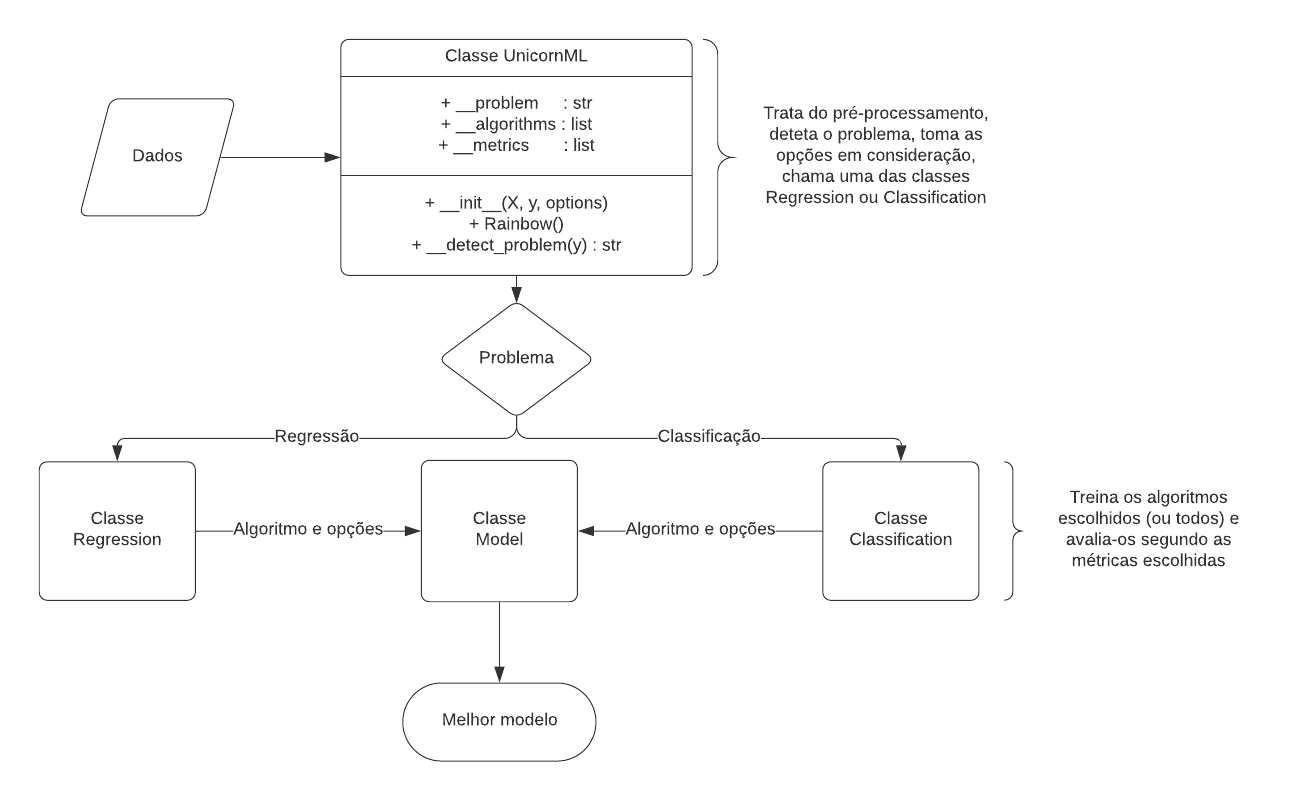
\includegraphics[width=1.0\textwidth]{Images/Diagram.png}
			\caption{Fluxo de execução da \textit{framework}}
			\label{fig:3}
		\end{figure}

		\subsection{Pré-processamento} \label{subsec:Pre-Processing}
		Na classe de pré-processamento realizam-se várias tarefas sobre os conjuntos de dados disponibilizados.
		Exibem-se de seguida as mesmas:

		\begin{itemize}
			\item Transformação dos dados:
			\begin{itemize}
				\item Separação entre os dados relativos às variáveis independentes dos dados associados à variável de interesse ou de saída;
				\item Resolução de valores omissos: colunas com mais de 40\% de valores nulos são eliminadas. Os valores numéricos são substituídos pela média dos valores da coluna enquanto que os categóricos são alterados para a moda;
				\item Redimensionamento e normalização: utilização de mecanismos de \textit{scaling} e \textit{label encoding} da biblioteca \texttt{scikit-learn}.
			\end{itemize}
			\item Seleção de \textit{features}:
			\begin{itemize}
				\item Utilização do \textit{PCA} para obter os principais componentes das \textit{features} com maior correlação e, por isso, com maior relevância.
			\end{itemize}
			
		\end{itemize}

		\subsection{Problema} \label{subsec:Problem}
		Os problemas de aprendizagem supervisionada podem ser divididos em dois conjuntos: problemas de regressão e problemas de classificação.
		Como tal, é importante perceber-se qual dos dois problemas enfrentamos, de forma a que se possa poupar tempo e recursos de computação na procura do melhor modelo.
		Para isso, foi pensada uma forma de identificar o tipo do problema. No entanto, tal como referido na proposta já entregue, esta não é uma prioridade,
		pelo que o método para já utilizado é simples e identifica apenas a presença de inteiros ou \textit{floats} para fazer esta distinção.

		No entanto, este processamento é evitado se o utilizador indicar qual dos problemas os seus dados representam.
		Esta indicação é dada através de uma opção, sendo passada uma de duas \textit{strings}: \textit{\texttt{Regression}} ou \textit{\texttt{Classification}}.

		\subsection{Algoritmos} \label{subsec:Algorithms}
		A \textsl{UnicornML} oferece diversos algoritmos para cada um dos tipos de problemas. 
		O utilizador pode escolher, dentro dos algoritmos disponíveis, quais os que quer que sejam testados. 
		No entanto, os algoritmos só serão testados se estiverem disponíveis para o tipo de problema identificado pela \textit{framework} ou indicado pelo mesmo.

		Caso o utilizador não indique quais os algoritmos que prefere que sejam testados, a \textit{framework} testará todos os algoritmos disponíveis para o tipo de problema identificado pela mesma ou indicado pelo utilizador.
            
			\subsubsection{Classificação} \label{sssec:Classification1}
			Os algoritmos disponíveis para problemas de classificação são os seguintes:
			\begin{itemize}
				\item Regressão logística;
				\item \textit{K-Nearest Neighbors} (KNN);
				\item \textit{Support Vector Classifier} (SVC) - uma \textit{Support Vector Machine} (SVM) para classificação;
				\item \textit{kernel} SVM - uma SVM com uma função \textit{kernel}, que permite a classificação em espaços de dimensão superiores;
				\item Classificadores Bayesianos - família de classificadores baseados na teoria de Bayes. Foram implementados quatro algoritmos diferentes: \textit{Gaussian}, \textit{Multinomial}, \textit{Bernoulli} e \textit{Complement};
				\item Árvores de decisão;
				\item \textit{Random Forest} - operam construindo uma multitude de árvores de decisão.
				\item Redes neuronais artificiais.
			\end{itemize}

			Estes algoritmos encontram-se na classe \texttt{Regression}, tal como se pode observar na figura \hyperref[fig:1]{1}.

			\subsubsection{Regressão} \label{sssec:Regression1}
			Os algoritmos disponíveis para problemas de regressão são os seguintes:
			\begin{itemize}
				\item Regressão linear;
				\item Regressão polinomial - os polinómios testados variam entre grau 2 e grau igual ao número de colunas da base de dados;
				\item \textit{Support Vector Regressor} (SVR) - uma SVM para regressão;
				\item Árvores de decisão;
				\item \textit{Random Forest} - operam construindo uma multitude de árvores de decisão;
				\item Redes neuronais artificiais.
			\end{itemize}

			Estes algoritmos encontram-se na classe \texttt{Classification}, presente na estrutura da \textit{framework} desta aplicação (consultar a figura \hyperref[fig:1]{1}).

		\subsection{Métricas} \label{subsec:Metrics}
		As métricas permitem avaliar o desempenho de um certo modelo. 
		O utilizador também pode escolher as métricas que irão ser tomadas em consideração e, posteriormente, apresentadas.
		Mais uma vez, isso está limitado às métricas disponíveis para cada tipo de problema.
		De realçar que nem todas as métricas podem estar disponíveis num determinado momento.

            \subsubsection{Classificação} \label{sssec:Classification2}
			As métricas disponíveis para problemas de classificação são as seguintes:
			\begin{itemize}
				\item \textit{Accuracy} - Percentagem de exemplos corretamente classificados (PECC). Esta métrica foi definida por omissão;
				\item \textit{Auc};
				\item \textit{Precision} - Valor preditivo positivo;
				\item \textit{Recall} - Sensibilidade.
			\end{itemize}

            \subsubsection{Regressão} \label{sssec:Regression2}
			As métricas disponíveis para problemas de regressão são as seguintes:
			\begin{itemize}
				\item \textit{Mean Square Error} (MSE) - métrica definida por omissão;
				\item \textit{Mean Absolute Error} (MAE);
				\item \textit{R-squared} ($R^{2}$).
			\end{itemize}

		\subsection{Modelo}
		A classe \texttt{Model}, em \texttt{unicornML/model/\_\_init\_\_.py}, é o coração de toda a \textit{framework}.
		Esta classe é utilizada tanto pela classe \texttt{Regression} como pela classe \texttt{Classification}.
		A mesma foi pensada de forma a simplificar o restante código e reduzir duplicações do mesmo.
		Nesta são incorporados vários tipos de informação, nomeadamente o conjunto de dados (treino e teste), a métrica selecionada para realizar a estimação do erro associada ao modelo escolhido e, ainda, os resultados obtidos após efetuar a otimização dos hiperparâmetros.

			\subsubsection{Otimização de hiperparâmetros} \label{sssec:Optimization}
			Tal como foi referido anteriormente, é nesta classe onde é realizada a procura do melhor modelo, segundo as opções escolhidas pelo utilizador.
			Para desempenhar a otimização de hiperparâmetros dos modelos considerados, o utilizador desta \textit{framework} de \textit{AutoML} pode indicar qual a otimização que pretende realizar.
			Nesta tomada de decisão este pode explicitamente indicar que não quer realizar tal tarefa. Por omissão, é realizada uma procura aleatória dos melhores parâmetros (\textit{RandomizedSearch}).
}

\chapter{Testes e análise de resultados} \label{ch:Test&Analysis}
\large{
	Para validar todos os aspetos considerados durante a implementação deste trabalho, foram incorporados nesta \textit{framework} vários conjuntos de dados que servem de teste à mesma.
	Como tal, foram adicionados no total 12 conjuntos de dados distintos entre si, havendo tanto problemas de regressão como de classificação a serem modelados.

}

\chapter{Conclusão} \label{ch:Conclusion}
\large{
	Será um pouco prematuro tentar tirar ilações de um trabalho incompleto, pelo que esta conclusão permite apenas refletir sobre as perspetivas existentes, tendo em conta o trabalho desenvolvido até agora.
	No entanto, é possível perceber que a \textsl{UnicornML} está no bom caminho, tendo em conta os resultados obtidos para os métodos já implementados e a ideia do que será possível ainda desenvolver.
}

\appendix
\chapter{Observações} \label{ch:Observations}
\begin{itemize}
    \item Documentação \textit{Python} 3:
	\par \textit{\url{https://docs.python.org/3/}}
	\item Documentação \textit{Pandas}:
	\par \textit{\url{https://pandas.pydata.org/docs/}}
	\item Documentação \textit{Numpy}:
	\par \textit{\url{https://numpy.org/doc/}}
	\item Documentação \textit{scikit-learn} - API:
    \par \textit{\url{https://scikit-learn.org/stable/modules/classes.html}}
	\item Documentação \textit{scikit-learn} - \textit{supervised learning}:
	\par \textit{\url{https://scikit-learn.org/stable/supervised_learning.html\#supervised-learning}}
\end{itemize}

\end{document}